\documentclass[ignorenonframetext,]{beamer}
\setbeamertemplate{caption}[numbered]
\setbeamertemplate{caption label separator}{: }
\setbeamercolor{caption name}{fg=normal text.fg}
\beamertemplatenavigationsymbolsempty
\usepackage{lmodern}
\usepackage{amssymb,amsmath}
\usepackage{ifxetex,ifluatex}
\usepackage{fixltx2e} % provides \textsubscript
\ifnum 0\ifxetex 1\fi\ifluatex 1\fi=0 % if pdftex
  \usepackage[T1]{fontenc}
  \usepackage[utf8]{inputenc}
\else % if luatex or xelatex
  \ifxetex
    \usepackage{mathspec}
  \else
    \usepackage{fontspec}
  \fi
  \defaultfontfeatures{Ligatures=TeX,Scale=MatchLowercase}
\fi
\usetheme[]{Darmstadt}
\usefonttheme{structurebold}
% use upquote if available, for straight quotes in verbatim environments
\IfFileExists{upquote.sty}{\usepackage{upquote}}{}
% use microtype if available
\IfFileExists{microtype.sty}{%
\usepackage{microtype}
\UseMicrotypeSet[protrusion]{basicmath} % disable protrusion for tt fonts
}{}
\newif\ifbibliography
\hypersetup{
            pdftitle={Operaciones, extración y otras funcionalidades entre tipos de estructuras de datos},
            pdfauthor={Santiago Lozano},
            pdfborder={0 0 0},
            breaklinks=true}
\urlstyle{same}  % don't use monospace font for urls
\usepackage{color}
\usepackage{fancyvrb}
\newcommand{\VerbBar}{|}
\newcommand{\VERB}{\Verb[commandchars=\\\{\}]}
\DefineVerbatimEnvironment{Highlighting}{Verbatim}{commandchars=\\\{\}}
% Add ',fontsize=\small' for more characters per line
\usepackage{framed}
\definecolor{shadecolor}{RGB}{248,248,248}
\newenvironment{Shaded}{\begin{snugshade}}{\end{snugshade}}
\newcommand{\KeywordTok}[1]{\textcolor[rgb]{0.13,0.29,0.53}{\textbf{#1}}}
\newcommand{\DataTypeTok}[1]{\textcolor[rgb]{0.13,0.29,0.53}{#1}}
\newcommand{\DecValTok}[1]{\textcolor[rgb]{0.00,0.00,0.81}{#1}}
\newcommand{\BaseNTok}[1]{\textcolor[rgb]{0.00,0.00,0.81}{#1}}
\newcommand{\FloatTok}[1]{\textcolor[rgb]{0.00,0.00,0.81}{#1}}
\newcommand{\ConstantTok}[1]{\textcolor[rgb]{0.00,0.00,0.00}{#1}}
\newcommand{\CharTok}[1]{\textcolor[rgb]{0.31,0.60,0.02}{#1}}
\newcommand{\SpecialCharTok}[1]{\textcolor[rgb]{0.00,0.00,0.00}{#1}}
\newcommand{\StringTok}[1]{\textcolor[rgb]{0.31,0.60,0.02}{#1}}
\newcommand{\VerbatimStringTok}[1]{\textcolor[rgb]{0.31,0.60,0.02}{#1}}
\newcommand{\SpecialStringTok}[1]{\textcolor[rgb]{0.31,0.60,0.02}{#1}}
\newcommand{\ImportTok}[1]{#1}
\newcommand{\CommentTok}[1]{\textcolor[rgb]{0.56,0.35,0.01}{\textit{#1}}}
\newcommand{\DocumentationTok}[1]{\textcolor[rgb]{0.56,0.35,0.01}{\textbf{\textit{#1}}}}
\newcommand{\AnnotationTok}[1]{\textcolor[rgb]{0.56,0.35,0.01}{\textbf{\textit{#1}}}}
\newcommand{\CommentVarTok}[1]{\textcolor[rgb]{0.56,0.35,0.01}{\textbf{\textit{#1}}}}
\newcommand{\OtherTok}[1]{\textcolor[rgb]{0.56,0.35,0.01}{#1}}
\newcommand{\FunctionTok}[1]{\textcolor[rgb]{0.00,0.00,0.00}{#1}}
\newcommand{\VariableTok}[1]{\textcolor[rgb]{0.00,0.00,0.00}{#1}}
\newcommand{\ControlFlowTok}[1]{\textcolor[rgb]{0.13,0.29,0.53}{\textbf{#1}}}
\newcommand{\OperatorTok}[1]{\textcolor[rgb]{0.81,0.36,0.00}{\textbf{#1}}}
\newcommand{\BuiltInTok}[1]{#1}
\newcommand{\ExtensionTok}[1]{#1}
\newcommand{\PreprocessorTok}[1]{\textcolor[rgb]{0.56,0.35,0.01}{\textit{#1}}}
\newcommand{\AttributeTok}[1]{\textcolor[rgb]{0.77,0.63,0.00}{#1}}
\newcommand{\RegionMarkerTok}[1]{#1}
\newcommand{\InformationTok}[1]{\textcolor[rgb]{0.56,0.35,0.01}{\textbf{\textit{#1}}}}
\newcommand{\WarningTok}[1]{\textcolor[rgb]{0.56,0.35,0.01}{\textbf{\textit{#1}}}}
\newcommand{\AlertTok}[1]{\textcolor[rgb]{0.94,0.16,0.16}{#1}}
\newcommand{\ErrorTok}[1]{\textcolor[rgb]{0.64,0.00,0.00}{\textbf{#1}}}
\newcommand{\NormalTok}[1]{#1}

% Prevent slide breaks in the middle of a paragraph:
\widowpenalties 1 10000
\raggedbottom

\AtBeginPart{
  \let\insertpartnumber\relax
  \let\partname\relax
  \frame{\partpage}
}
\AtBeginSection{
  \ifbibliography
  \else
    \let\insertsectionnumber\relax
    \let\sectionname\relax
    \frame{\sectionpage}
  \fi
}
\AtBeginSubsection{
  \let\insertsubsectionnumber\relax
  \let\subsectionname\relax
  \frame{\subsectionpage}
}

\setlength{\parindent}{0pt}
\setlength{\parskip}{6pt plus 2pt minus 1pt}
\setlength{\emergencystretch}{3em}  % prevent overfull lines
\providecommand{\tightlist}{%
  \setlength{\itemsep}{0pt}\setlength{\parskip}{0pt}}
\setcounter{secnumdepth}{0}

\title{Operaciones, extración y otras funcionalidades entre tipos de
estructuras de datos}
\author{Santiago Lozano}
\date{21 de febrero de 2020}

\begin{document}
\frame{\titlepage}

\begin{frame}[fragile]{Evaluación de combinaciones de TRUE o FALSE}

Es importante saber cómo se operan los conectores lógicos
vistos anteriormente, referente a los distintos valores logical que
pueden resultar, además de cómo se operan los Missing Values con los
otros valores lógicos, veamos todas las combinaciones mediante la
siguiente codificación

\begin{Shaded}
\begin{Highlighting}[]
\NormalTok{x <-}\StringTok{ }\KeywordTok{c}\NormalTok{(}\OtherTok{NA}\NormalTok{, }\OtherTok{FALSE}\NormalTok{, }\OtherTok{TRUE}\NormalTok{)}
\KeywordTok{names}\NormalTok{(x) <-}\StringTok{ }\KeywordTok{as.character}\NormalTok{(x)}
\NormalTok{x}
\end{Highlighting}
\end{Shaded}

\begin{verbatim}
##  <NA> FALSE  TRUE 
##    NA FALSE  TRUE
\end{verbatim}

\end{frame}

\begin{frame}[fragile]{Evaluación de combinaciones de TRUE o FALSE}

Veamos las distintas combinaciones mediante el conector lógico y (\&)

\begin{Shaded}
\begin{Highlighting}[]
\KeywordTok{outer}\NormalTok{(x, x, }\StringTok{"&"}\NormalTok{)}
\end{Highlighting}
\end{Shaded}

\begin{verbatim}
##        <NA> FALSE  TRUE
## <NA>     NA FALSE    NA
## FALSE FALSE FALSE FALSE
## TRUE     NA FALSE  TRUE
\end{verbatim}

\end{frame}

\begin{frame}[fragile]{Evaluación de combinaciones de TRUE o FALSE}

Ahora mediante el conector ó (\textbar{})

\begin{Shaded}
\begin{Highlighting}[]
\KeywordTok{outer}\NormalTok{(x, x, }\StringTok{"|"}\NormalTok{)}
\end{Highlighting}
\end{Shaded}

\begin{verbatim}
##       <NA> FALSE TRUE
## <NA>    NA    NA TRUE
## FALSE   NA FALSE TRUE
## TRUE  TRUE  TRUE TRUE
\end{verbatim}

\end{frame}

\begin{frame}[fragile]{Lógica Aritmética}

La aritmética que envuelven las expresiones lógica las diferentes
estrucutras de datos juega un papel muy importante a la hora de
programar nos indicará de una u otra forma que elementos escoger y
cuales no, la clave para entende esta parte es que las expresiones
lógicas evaluan si es cierto o falso alguna proposición, y qué R puede
convertir en valores numéricos 1 para TRUE, 0 para FALSE

\begin{Shaded}
\begin{Highlighting}[]
\NormalTok{x<-}\StringTok{ }\DecValTok{0}\OperatorTok{:}\DecValTok{6}
\end{Highlighting}
\end{Shaded}

\begin{Shaded}
\begin{Highlighting}[]
\NormalTok{x }\OperatorTok{<}\StringTok{ }\DecValTok{4}
\end{Highlighting}
\end{Shaded}

\begin{verbatim}
## [1]  TRUE  TRUE  TRUE  TRUE FALSE FALSE FALSE
\end{verbatim}

\end{frame}

\begin{frame}[fragile]{Lógica Aritmética}

Para poder chequear si todos los valores de un vector cumplen con la
condición o para verificar si alguno cumple la condición usamos all() y
any()

\begin{Shaded}
\begin{Highlighting}[]
\KeywordTok{all}\NormalTok{(x}\OperatorTok{>}\DecValTok{0}\NormalTok{)}
\end{Highlighting}
\end{Shaded}

\begin{verbatim}
## [1] FALSE
\end{verbatim}

\begin{Shaded}
\begin{Highlighting}[]
\KeywordTok{any}\NormalTok{(x}\OperatorTok{<}\DecValTok{0}\NormalTok{)}
\end{Highlighting}
\end{Shaded}

\begin{verbatim}
## [1] FALSE
\end{verbatim}

\end{frame}

\begin{frame}[fragile]{Lógica Aritmética}

Podemos usar las respuestas de las funciones lógicas en aritmética.
Podemos contar los valores TRUE de (x\textless{}4), usando sum

\begin{Shaded}
\begin{Highlighting}[]
\KeywordTok{sum}\NormalTok{(x}\OperatorTok{<}\DecValTok{4}\NormalTok{)}
\end{Highlighting}
\end{Shaded}

\begin{verbatim}
## [1] 4
\end{verbatim}

Podemos multiplicar el vector (x\textless{}4) por otros vectores

\begin{Shaded}
\begin{Highlighting}[]
\NormalTok{(x}\OperatorTok{<}\DecValTok{4}\NormalTok{)}\OperatorTok{*}\KeywordTok{runif}\NormalTok{(}\DecValTok{7}\NormalTok{)}
\end{Highlighting}
\end{Shaded}

\begin{verbatim}
## [1] 0.2541504 0.3750152 0.9489598 0.6974481 0.0000000
## [6] 0.0000000 0.0000000
\end{verbatim}

\end{frame}

\begin{frame}[fragile]{Lógica Aritmética}

\begin{Shaded}
\begin{Highlighting}[]
\NormalTok{y <-}\StringTok{ }\KeywordTok{c}\NormalTok{(}\DecValTok{4}\NormalTok{,}\OtherTok{NA}\NormalTok{,}\DecValTok{7}\NormalTok{)}
\NormalTok{y }\OperatorTok{==}\StringTok{ }\OtherTok{NA} \CommentTok{# no funciona}
\end{Highlighting}
\end{Shaded}

\begin{verbatim}
## [1] NA NA NA
\end{verbatim}

U

\begin{Shaded}
\begin{Highlighting}[]
\NormalTok{y }\OperatorTok{==}\StringTok{ "NA"} \CommentTok{# no funciona}
\end{Highlighting}
\end{Shaded}

\begin{verbatim}
## [1] FALSE    NA FALSE
\end{verbatim}

\begin{Shaded}
\begin{Highlighting}[]
\KeywordTok{is.na}\NormalTok{(y)}
\end{Highlighting}
\end{Shaded}

\begin{verbatim}
## [1] FALSE  TRUE FALSE
\end{verbatim}

\end{frame}

\begin{frame}[fragile]{Lógica Aritmética}

La lógica aritmética es útil para generar niveles simplificados de
factores durante el modelamiento estadístico. Suponga que queremos
reducir un factor de 5 niveles (a, b, c, d, e) llamado tratamiento a un
factor de 3 niveles llamado t2 juntados los niveles a y e (nuevo factor
nivel 1) y c y d (nuevo factor nivel 3) mientras que dejamos b solo
(nuevo factor nivel 2)

\begin{Shaded}
\begin{Highlighting}[]
\NormalTok{tratamiento <-}\StringTok{ }\NormalTok{letters[}\DecValTok{1}\OperatorTok{:}\DecValTok{5}\NormalTok{]}
\NormalTok{tratamiento}
\end{Highlighting}
\end{Shaded}

\begin{verbatim}
## [1] "a" "b" "c" "d" "e"
\end{verbatim}

\begin{Shaded}
\begin{Highlighting}[]
\DecValTok{1} \OperatorTok{+}\StringTok{ }\NormalTok{(tratamiento }\OperatorTok{==}\StringTok{ "b"}\NormalTok{)}
\end{Highlighting}
\end{Shaded}

\begin{verbatim}
## [1] 1 2 1 1 1
\end{verbatim}

\end{frame}

\begin{frame}[fragile]{Lógica Aritmética}

\begin{Shaded}
\begin{Highlighting}[]
\NormalTok{t2 <-}\StringTok{ }\KeywordTok{factor}\NormalTok{(}\DecValTok{1}\OperatorTok{+}\NormalTok{(tratamiento}\OperatorTok{==}\StringTok{"b"}\NormalTok{)}\OperatorTok{+}\DecValTok{2}\OperatorTok{*}\NormalTok{(tratamiento}\OperatorTok{==}\StringTok{"c"}\NormalTok{)}
             \OperatorTok{+}\DecValTok{2}\OperatorTok{*}\NormalTok{(tratamiento}\OperatorTok{==}\StringTok{"d"}\NormalTok{))}
\NormalTok{t2}
\end{Highlighting}
\end{Shaded}

\begin{verbatim}
## [1] 1 2 3 3 1
## Levels: 1 2 3
\end{verbatim}

\end{frame}

\begin{frame}[fragile]{Distinciones entre las igualdades}

\texttt{x\ \textless{}-\ y} a x le asigno el valor de y

\texttt{x\ =\ y} en una función o una lista x se establece en y, a menos
que especifique lo contrario

\texttt{x\ ==\ y} produce TRUE si x es exactamente igual a y y falso en
otro caso

\end{frame}

\begin{frame}[fragile]{Resumén de diferencias entre objetos usando
all.equal}

La función all.equal es muy útil in programación para chequear que los
objetos son realmente como tu esperabas. Cuando ocurren diferencias,
all.equal hace un trabajo útil en describir todas las diferencias
encontradas

\begin{Shaded}
\begin{Highlighting}[]
\NormalTok{a <-}\StringTok{ }\KeywordTok{c}\NormalTok{(}\StringTok{"cat"}\NormalTok{,}\StringTok{"dog"}\NormalTok{,}\StringTok{"goldfish"}\NormalTok{)}
\NormalTok{b <-}\StringTok{ }\KeywordTok{factor}\NormalTok{(a)}
\end{Highlighting}
\end{Shaded}

\begin{Shaded}
\begin{Highlighting}[]
\KeywordTok{all.equal}\NormalTok{(a,b)}
\end{Highlighting}
\end{Shaded}

\begin{verbatim}
## [1] "Modes: character, numeric"                      
## [2] "Attributes: < target is NULL, current is list >"
## [3] "target is character, current is factor"
\end{verbatim}

\end{frame}

\begin{frame}[fragile]{Resumen de diferencias entre objetos usando
all.equal}

en este caso el objeto de la izquierda (a) es llamado ``target'' y el
objeto de la derecha (b) es ``current''

\begin{Shaded}
\begin{Highlighting}[]
\KeywordTok{mode}\NormalTok{(b)}
\end{Highlighting}
\end{Shaded}

\begin{verbatim}
## [1] "numeric"
\end{verbatim}

\begin{Shaded}
\begin{Highlighting}[]
\KeywordTok{mode}\NormalTok{(a)}
\end{Highlighting}
\end{Shaded}

\begin{verbatim}
## [1] "character"
\end{verbatim}

\end{frame}

\begin{frame}[fragile]{Resumen de diferencias entre objetos usando
all.equal}

\begin{Shaded}
\begin{Highlighting}[]
\KeywordTok{attributes}\NormalTok{(b)}
\end{Highlighting}
\end{Shaded}

\begin{verbatim}
## $levels
## [1] "cat"      "dog"      "goldfish"
## 
## $class
## [1] "factor"
\end{verbatim}

\begin{Shaded}
\begin{Highlighting}[]
\KeywordTok{attributes}\NormalTok{(a)}
\end{Highlighting}
\end{Shaded}

\begin{verbatim}
## NULL
\end{verbatim}

\end{frame}

\begin{frame}[fragile]{Resumén de diferencias entre objetos usando
all.equal}

\begin{Shaded}
\begin{Highlighting}[]
\NormalTok{n1 <-}\StringTok{ }\KeywordTok{c}\NormalTok{(}\DecValTok{1}\NormalTok{,}\DecValTok{2}\NormalTok{,}\DecValTok{3}\NormalTok{)}
\NormalTok{n2 <-}\StringTok{ }\KeywordTok{c}\NormalTok{(}\DecValTok{1}\NormalTok{,}\DecValTok{2}\NormalTok{,}\DecValTok{3}\NormalTok{,}\DecValTok{4}\NormalTok{)}
\KeywordTok{all.equal}\NormalTok{(n1,n2)}
\end{Highlighting}
\end{Shaded}

\begin{verbatim}
## [1] "Numeric: lengths (3, 4) differ"
\end{verbatim}

\begin{Shaded}
\begin{Highlighting}[]
\NormalTok{n2 <-}\StringTok{ }\KeywordTok{as.character}\NormalTok{(n2)}
\KeywordTok{all.equal}\NormalTok{(n1,n2)}
\end{Highlighting}
\end{Shaded}

\begin{verbatim}
## [1] "Modes: numeric, character"              
## [2] "Lengths: 3, 4"                          
## [3] "target is numeric, current is character"
\end{verbatim}

\end{frame}

\begin{frame}[fragile]{Funciones básicas para vectores}

Una de las fortalezas de R es la habilidad de evaluar funciones sobre
vectores enteros, con gran utilidad a la hora de operar ciclos, veamos
algunas de las funciones más importantes, la mayoría de las funciones
aplican para vectores de tipo numeric

\begin{Shaded}
\begin{Highlighting}[]
\NormalTok{y <-}\StringTok{ }\KeywordTok{c}\NormalTok{(}\DecValTok{8}\NormalTok{,}\DecValTok{3}\NormalTok{,}\DecValTok{5}\NormalTok{,}\DecValTok{7}\NormalTok{,}\DecValTok{6}\NormalTok{,}\DecValTok{6}\NormalTok{,}\DecValTok{8}\NormalTok{,}\DecValTok{9}\NormalTok{,}\DecValTok{2}\NormalTok{,}\DecValTok{3}\NormalTok{,}\DecValTok{9}\NormalTok{,}\DecValTok{4}\NormalTok{,}\DecValTok{10}\NormalTok{,}\DecValTok{4}\NormalTok{,}\DecValTok{11}\NormalTok{)}
\end{Highlighting}
\end{Shaded}

función media

\begin{Shaded}
\begin{Highlighting}[]
\KeywordTok{mean}\NormalTok{(y)}
\end{Highlighting}
\end{Shaded}

\begin{verbatim}
## [1] 6.333333
\end{verbatim}

\end{frame}

\begin{frame}[fragile]{Funciones básicas para vectores}

Largo de un vector

\begin{Shaded}
\begin{Highlighting}[]
\KeywordTok{length}\NormalTok{(y)}
\end{Highlighting}
\end{Shaded}

\begin{verbatim}
## [1] 15
\end{verbatim}

rango de los números en un vector

\begin{Shaded}
\begin{Highlighting}[]
\KeywordTok{range}\NormalTok{(y)}
\end{Highlighting}
\end{Shaded}

\begin{verbatim}
## [1]  2 11
\end{verbatim}

\end{frame}

\begin{frame}[fragile]{Funciones básicas para vectores}

ordenar los elementos del vector de menor a mayor

\begin{Shaded}
\begin{Highlighting}[]
\KeywordTok{sort}\NormalTok{(y)}
\end{Highlighting}
\end{Shaded}

\begin{verbatim}
##  [1]  2  3  3  4  4  5  6  6  7  8  8  9  9 10 11
\end{verbatim}

de forma decreciente

\begin{Shaded}
\begin{Highlighting}[]
\KeywordTok{sort}\NormalTok{(y,}\DataTypeTok{decreasing =} \OtherTok{TRUE}\NormalTok{)}
\end{Highlighting}
\end{Shaded}

\begin{verbatim}
##  [1] 11 10  9  9  8  8  7  6  6  5  4  4  3  3  2
\end{verbatim}

\end{frame}

\begin{frame}[fragile]{Funciones básicas para vectores}

reodernar los elementos del vector en order reversivo

\begin{Shaded}
\begin{Highlighting}[]
\KeywordTok{rev}\NormalTok{(y)}
\end{Highlighting}
\end{Shaded}

\begin{verbatim}
##  [1] 11  4 10  4  9  3  2  9  8  6  6  7  5  3  8
\end{verbatim}

remover los duplicados en un vector

\begin{Shaded}
\begin{Highlighting}[]
\KeywordTok{unique}\NormalTok{(y)}
\end{Highlighting}
\end{Shaded}

\begin{verbatim}
##  [1]  8  3  5  7  6  9  2  4 10 11
\end{verbatim}

\end{frame}

\begin{frame}[fragile]{Funciones básicas para vectores}

valor lógico en cada elemento que afirma si está duplicado o no

\begin{Shaded}
\begin{Highlighting}[]
\KeywordTok{duplicated}\NormalTok{(y)}
\end{Highlighting}
\end{Shaded}

\begin{verbatim}
##  [1] FALSE FALSE FALSE FALSE FALSE  TRUE  TRUE
##  [8] FALSE FALSE  TRUE  TRUE  FALSE FALSE TRUE 
## [15] FALSE
\end{verbatim}

which indica que índice lleva el valor TRUE

\begin{Shaded}
\begin{Highlighting}[]
\NormalTok{mask <-}\StringTok{ }\KeywordTok{c}\NormalTok{(}\OtherTok{TRUE}\NormalTok{,}\OtherTok{FALSE}\NormalTok{,}\OtherTok{TRUE}\NormalTok{,}\OtherTok{NA}\NormalTok{,}\OtherTok{FALSE}\NormalTok{,}\OtherTok{FALSE}\NormalTok{,}\OtherTok{TRUE}\NormalTok{)}
\KeywordTok{which}\NormalTok{(mask)}
\end{Highlighting}
\end{Shaded}

\begin{verbatim}
## [1] 1 3 7
\end{verbatim}

\end{frame}

\begin{frame}[fragile]{Funciones básicas para vectores}

Para buscar el índice con el menor valor

\begin{Shaded}
\begin{Highlighting}[]
\KeywordTok{which.min}\NormalTok{(y)}
\end{Highlighting}
\end{Shaded}

\begin{verbatim}
## [1] 9
\end{verbatim}

ahora con el mayor valor

\begin{Shaded}
\begin{Highlighting}[]
\KeywordTok{which.max}\NormalTok{(y)}
\end{Highlighting}
\end{Shaded}

\begin{verbatim}
## [1] 15
\end{verbatim}

\end{frame}

\begin{frame}[fragile]{Funciones básicas para vectores}

para nombrar los elementos de un vector

\begin{Shaded}
\begin{Highlighting}[]
\KeywordTok{names}\NormalTok{(y) <-}\StringTok{ }\DecValTok{1}\OperatorTok{:}\DecValTok{15}
\NormalTok{y}
\end{Highlighting}
\end{Shaded}

\begin{verbatim}
##  1  2  3  4  5  6  7  8  9 10 11 12 13 14 15 
##  8  3  5  7  6  6  8  9  2  3  9  4 10  4 11
\end{verbatim}

La suma acumulada

\begin{Shaded}
\begin{Highlighting}[]
\KeywordTok{cumsum}\NormalTok{(y)}
\end{Highlighting}
\end{Shaded}

\begin{verbatim}
##  1  2  3  4  5  6  7  8  9 10 11 12 13 14 15 
##  8 11 16 23 29 35 43 52 54 57 66 70 80 84 95
\end{verbatim}

\end{frame}

\begin{frame}[fragile]{Funciones básicas para vectores}

El producto acumulado

\begin{Shaded}
\begin{Highlighting}[]
\KeywordTok{cumprod}\NormalTok{(y)}
\end{Highlighting}
\end{Shaded}

\begin{verbatim}
##        1         2          3           4            5 
##        8        24        120         840         5040 
##        6         7          8            9          10 
##    30240    241920    2177280     4354560     13063680 
##       11        12         13           14          15 
##117573120 470292480 4702924800 18811699200 206928691200
\end{verbatim}

\end{frame}

\begin{frame}[fragile]{Funciones básicas para vectores}

mínimo

\begin{Shaded}
\begin{Highlighting}[]
\KeywordTok{min}\NormalTok{(y)}
\end{Highlighting}
\end{Shaded}

\begin{verbatim}
## [1] 2
\end{verbatim}

\begin{Shaded}
\begin{Highlighting}[]
\KeywordTok{max}\NormalTok{(y)}
\end{Highlighting}
\end{Shaded}

\begin{verbatim}
## [1] 11
\end{verbatim}

\begin{Shaded}
\begin{Highlighting}[]
\KeywordTok{quantile}\NormalTok{(y)}
\end{Highlighting}
\end{Shaded}

\begin{verbatim}
##   0%  25%  50%  75% 100% 
##  2.0  4.0  6.0  8.5 11.0
\end{verbatim}

\end{frame}

\begin{frame}[fragile]{Funciones básicas para vectores}

con pmin y pmax tomamos tres vectores con el mismo largor y hallamos el
valor mínimo de cada componente

\begin{Shaded}
\begin{Highlighting}[]
\NormalTok{x<-}\KeywordTok{c}\NormalTok{(}\FloatTok{0.99}\NormalTok{,}\FloatTok{0.98}\NormalTok{,}\FloatTok{0.20}\NormalTok{,}\FloatTok{0.65}\NormalTok{,}\FloatTok{0.93}\NormalTok{,}\FloatTok{0.18}\NormalTok{)}
\NormalTok{x}
\end{Highlighting}
\end{Shaded}

\begin{verbatim}
## [1] 0.99 0.98 0.20 0.65 0.93 0.18
\end{verbatim}

\begin{Shaded}
\begin{Highlighting}[]
\NormalTok{y<-}\KeywordTok{c}\NormalTok{(}\FloatTok{0.51}\NormalTok{,}\FloatTok{0.30}\NormalTok{,}\FloatTok{0.41}\NormalTok{,}\FloatTok{0.53}\NormalTok{,}\FloatTok{0.07}\NormalTok{,}\FloatTok{0.49}\NormalTok{)}
\NormalTok{y}
\end{Highlighting}
\end{Shaded}

\begin{verbatim}
## [1] 0.51 0.30 0.41 0.53 0.07 0.49
\end{verbatim}

\end{frame}

\begin{frame}[fragile]{Funciones básicas para vectores}

\begin{Shaded}
\begin{Highlighting}[]
\NormalTok{z<-}\KeywordTok{c}\NormalTok{(}\FloatTok{0.26}\NormalTok{,}\FloatTok{0.132}\NormalTok{,}\FloatTok{0.44}\NormalTok{,}\FloatTok{0.65}\NormalTok{,}\FloatTok{0.031}\NormalTok{,}\FloatTok{0.36}\NormalTok{)}
\NormalTok{z}
\end{Highlighting}
\end{Shaded}

\begin{verbatim}
## [1] 0.260 0.132 0.440 0.650 0.031 0.360
\end{verbatim}

\begin{Shaded}
\begin{Highlighting}[]
\KeywordTok{pmin}\NormalTok{(x,y,z)}
\end{Highlighting}
\end{Shaded}

\begin{verbatim}
## [1] 0.260 0.132 0.200 0.530 0.031 0.180
\end{verbatim}

\end{frame}

\begin{frame}[fragile]{Funciones básicas para vectores}

para contar la cantidad el número de elementos de cada componente del
vector

\begin{Shaded}
\begin{Highlighting}[]
\KeywordTok{table}\NormalTok{(y)}
\end{Highlighting}
\end{Shaded}

\begin{verbatim}
## y
## 0.07  0.3 0.41 0.49 0.51 0.53 
##    1    1    1    1    1    1
\end{verbatim}

ordena los elementos pero despliega los índices

\end{frame}

\begin{frame}[fragile]{Funciones básicas para vectores}

\begin{Shaded}
\begin{Highlighting}[]
\NormalTok{y <-}\StringTok{ }\KeywordTok{c}\NormalTok{(}\DecValTok{8}\NormalTok{,}\DecValTok{3}\NormalTok{,}\DecValTok{5}\NormalTok{,}\DecValTok{7}\NormalTok{,}\DecValTok{6}\NormalTok{,}\DecValTok{6}\NormalTok{,}\DecValTok{8}\NormalTok{,}\DecValTok{9}\NormalTok{,}\DecValTok{2}\NormalTok{,}\DecValTok{3}\NormalTok{,}\DecValTok{9}\NormalTok{,}\DecValTok{4}\NormalTok{,}\DecValTok{10}\NormalTok{,}\DecValTok{4}\NormalTok{,}\DecValTok{11}\NormalTok{)}
\end{Highlighting}
\end{Shaded}

\begin{Shaded}
\begin{Highlighting}[]
\KeywordTok{order}\NormalTok{(y)}
\end{Highlighting}
\end{Shaded}

\begin{verbatim}
##  [1]  9  2 10 12 14  3  5  6  4  1  7  8 11 13 15
\end{verbatim}

\end{frame}

\begin{frame}[fragile]{Funciones básicas sobre vectores}

\begin{Shaded}
\begin{Highlighting}[]
\KeywordTok{rank}\NormalTok{(y)}
\end{Highlighting}
\end{Shaded}

\begin{verbatim}
##  [1] 10.5  2.5  6.0  9.0  7.5  7.5 10.5 12.5  1.0
## [10] 2.5 12.5  4.5 14.0  4.5 15.0
\end{verbatim}

\end{frame}

\begin{frame}[fragile]{Funciones básicas sobre matrices y dataframes}

Tomemos la siguiente matriz

\begin{Shaded}
\begin{Highlighting}[]
\NormalTok{vector <-}\StringTok{ }\KeywordTok{c}\NormalTok{(}\DecValTok{1}\NormalTok{,}\DecValTok{2}\NormalTok{,}\DecValTok{3}\NormalTok{,}\DecValTok{4}\NormalTok{,}\DecValTok{4}\NormalTok{,}\DecValTok{3}\NormalTok{,}\DecValTok{2}\NormalTok{,}\DecValTok{1}\NormalTok{)}
\NormalTok{V <-}\StringTok{ }\KeywordTok{matrix}\NormalTok{(vector,}\DataTypeTok{byrow=}\NormalTok{T,}\DataTypeTok{nrow=}\DecValTok{2}\NormalTok{)}
\NormalTok{V}
\end{Highlighting}
\end{Shaded}

\begin{verbatim}
##      [,1] [,2] [,3] [,4]
## [1,]    1    2    3    4
## [2,]    4    3    2    1
\end{verbatim}

\begin{Shaded}
\begin{Highlighting}[]
\KeywordTok{dim}\NormalTok{(V)}
\end{Highlighting}
\end{Shaded}

\begin{verbatim}
## [1] 2 4
\end{verbatim}

\end{frame}

\begin{frame}[fragile]{Funciones básicas sobre matrices y dataframes}

\begin{Shaded}
\begin{Highlighting}[]
\KeywordTok{nrow}\NormalTok{(V)}
\end{Highlighting}
\end{Shaded}

\begin{verbatim}
## [1] 2
\end{verbatim}

\begin{Shaded}
\begin{Highlighting}[]
\KeywordTok{ncol}\NormalTok{(V)}
\end{Highlighting}
\end{Shaded}

\begin{verbatim}
## [1] 4
\end{verbatim}

\end{frame}

\begin{frame}[fragile]{Funciones básicas sobre matrices y dataframes}

\begin{Shaded}
\begin{Highlighting}[]
\KeywordTok{dimnames}\NormalTok{(V) <-}\StringTok{ }\KeywordTok{list}\NormalTok{(}\KeywordTok{c}\NormalTok{(}\StringTok{"ad"}\NormalTok{,}\StringTok{"sd"}\NormalTok{),}\KeywordTok{c}\NormalTok{(}\StringTok{"aa"}\NormalTok{,}\StringTok{"bb"}\NormalTok{,}\StringTok{"cc"}\NormalTok{,}\StringTok{" d"}\NormalTok{))}
\NormalTok{V          }
\end{Highlighting}
\end{Shaded}

\begin{verbatim}
##    aa bb cc  d
## ad  1  2  3  4
## sd  4  3  2  1
\end{verbatim}

names(), colnames(): nombres de columnas

rownames(): nombres de filas

\end{frame}

\begin{frame}{Funciones básicas}

\begin{center}
\begin{figure}
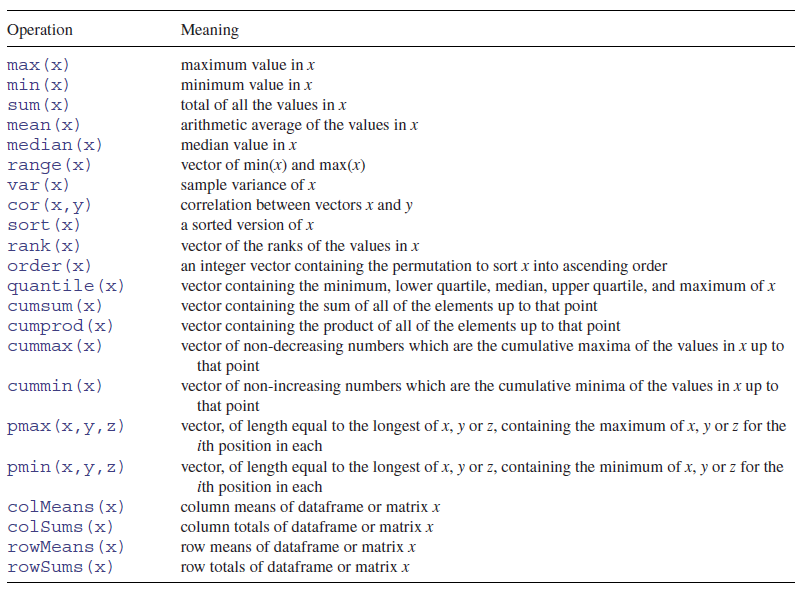
\includegraphics[scale=0.45]{vectores.png}
\end{figure}
\end{center}


\end{frame}

\begin{frame}[fragile]{Aplicación de funciones en masa para matrices,
dataframes y listas (apply())}

La función apply(), aplica una función dada (con el argumento FUN) a
todas la filas (MARGIN=1) o todas las columnas (MARGIN=2)

\begin{Shaded}
\begin{Highlighting}[]
\NormalTok{V <-}\StringTok{ }\KeywordTok{matrix}\NormalTok{(vector,}\DataTypeTok{byrow=}\NormalTok{T,}\DataTypeTok{nrow=}\DecValTok{2}\NormalTok{)}
\NormalTok{V}
\end{Highlighting}
\end{Shaded}

\begin{verbatim}
##      [,1] [,2] [,3] [,4]
## [1,]    1    2    3    4
## [2,]    4    3    2    1
\end{verbatim}

\begin{Shaded}
\begin{Highlighting}[]
\KeywordTok{apply}\NormalTok{(V,}\DataTypeTok{MARGIN =} \DecValTok{1}\NormalTok{,}\DataTypeTok{FUN =}\NormalTok{ mean)}
\end{Highlighting}
\end{Shaded}

\begin{verbatim}
## [1] 2.5 2.5
\end{verbatim}

\end{frame}

\begin{frame}[fragile]{Aplicación de funciones en masa para matrices,
dataframes y listas (apply())}

\begin{Shaded}
\begin{Highlighting}[]
\KeywordTok{apply}\NormalTok{(V,}\DataTypeTok{MARGIN =} \DecValTok{1}\NormalTok{,}\DataTypeTok{FUN =}\NormalTok{ sum)}
\end{Highlighting}
\end{Shaded}

\begin{verbatim}
## [1] 10 10
\end{verbatim}

\end{frame}

\begin{frame}{Hágalo usted mismo}

Vamos a calcular la suma cuadrada de todas las filas de una matriz M de
tamaño 5x2 con los número a bondad. Usando la función apply() sobre la
filas de la matriz, se usará el argumento asociado FUN=function(x)
\{sum(x\^{}2)\}

\end{frame}

\begin{frame}[fragile]{Función sweep()}

Esta función es muy útil para realizar un barrido (en el sentido de una
función por FUN) a cierto estadístico (dado por el argumento STATS),
para todas las filas (MARGIN=1) o todas las columnas (MARGIN=2)

\begin{Shaded}
\begin{Highlighting}[]
\NormalTok{V}
\end{Highlighting}
\end{Shaded}

\begin{verbatim}
##      [,1] [,2] [,3] [,4]
## [1,]    1    2    3    4
## [2,]    4    3    2    1
\end{verbatim}

\end{frame}

\begin{frame}[fragile]{Función sweep()}

vamos a restar 3 de la fila 1 y 5 de la fila 2

\begin{Shaded}
\begin{Highlighting}[]
\KeywordTok{sweep}\NormalTok{(V,}\DataTypeTok{MARGIN=}\DecValTok{1}\NormalTok{,}\DataTypeTok{STATS=}\KeywordTok{c}\NormalTok{(}\DecValTok{3}\NormalTok{,}\DecValTok{5}\NormalTok{),}\DataTypeTok{FUN=}\StringTok{"-"}\NormalTok{)}
\end{Highlighting}
\end{Shaded}

\begin{verbatim}
##      [,1] [,2] [,3] [,4]
## [1,]   -2   -1    0    1
## [2,]   -1   -2   -3   -4
\end{verbatim}

vamos a dividir las primeras dos columnas por 2 y las dos útilmas por 3

\begin{Shaded}
\begin{Highlighting}[]
\KeywordTok{sweep}\NormalTok{(V,}\DataTypeTok{MARGIN=}\DecValTok{2}\NormalTok{,}\DataTypeTok{STATS=}\KeywordTok{c}\NormalTok{(}\DecValTok{2}\NormalTok{,}\DecValTok{2}\NormalTok{,}\DecValTok{3}\NormalTok{,}\DecValTok{3}\NormalTok{),}\DataTypeTok{FUN=}\StringTok{"/"}\NormalTok{)}
\end{Highlighting}
\end{Shaded}

\begin{verbatim}
##      [,1] [,2]      [,3]      [,4]
## [1,]  0.5  1.0 1.0000000 1.3333333
## [2,]  2.0  1.5 0.6666667 0.3333333
\end{verbatim}

\end{frame}

\end{document}
